% -*- mode: LaTeX; TeX-PDF-mode: t; -*- 
% LaTeX path to the root directory of the current project
% from the directory in which this file resides
% and path to econtexPaths which defines the rest of the paths like \FigDir
\providecommand{\econtexRoot}{}\renewcommand{\econtexRoot}{.}
\providecommand{\econtexPaths}{}\renewcommand{\econtexPaths}{econtexPaths}
% -*- mode: LaTeX; TeX-PDF-mode: t; -*- 
% The \commands below are required to allow sharing of the same base code via Github between TeXLive on a local machine and Overleaf (which is a proxy for "a standard distribution of LaTeX").  This is an ugly solution to the requirement that custom LaTeX packages be accessible, and that Overleaf prohibits symbolic links
\providecommand{\packages}{\econtexRoot/Resources/texmf-local/tex/latex}
\providecommand{\econtex}{\packages/econtex}
\providecommand{\econark}{\econtexRoot/Resources/texmf-local/tex/latex/econark}
\providecommand{\econtexSetup}{\econtexRoot/Resources/texmf-local/tex/latex/econtexSetup}
\providecommand{\econarkSetup}{\econtexRoot/Resources/texmf-local/tex/latex/econarkSetup}
\providecommand{\econtexShortcuts}{\econtexRoot/Resources/texmf-local/tex/latex/econtexShortcuts}
\providecommand{\econtexBibMake}{\econtexRoot/Resources/texmf-local/tex/latex/econtexBibMake}
\providecommand{\econtexBibStyle}{\econtexRoot/Resources/texmf-local/bibtex/bst/econtex}
\providecommand{\econtexBib}{economics}
\providecommand{\notes}{\econtexRoot/Resources/texmf-local/tex/latex/handout}
\providecommand{\handoutSetup}{\econtexRoot/Resources/texmf-local/tex/latex/handoutSetup}
\providecommand{\handoutShortcuts}{\econtexRoot/Resources/texmf-local/tex/latex/handoutShortcuts}
\providecommand{\handoutBibMake}{\econtexRoot/Resources/texmf-local/tex/latex/handoutBibMake}
\providecommand{\handoutBibStyle}{\econtexRoot/Resources/texmf-local/bibtex/bst/handout}

\providecommand{\FigDir}{\econtexRoot/Figures}
\providecommand{\CodeDir}{\econtexRoot/Code}
\providecommand{\DataDir}{\econtexRoot/Data}
\providecommand{\SlideDir}{\econtexRoot/Slides}
\providecommand{\TableDir}{\econtexRoot/Tables}
\providecommand{\ApndxDir}{\econtexRoot/Appendices}

\providecommand{\ResourcesDir}{\econtexRoot/Resources}
\providecommand{\rootFromOut}{..} % APFach back to root directory from output-directory
\providecommand{\LaTeXGenerated}{\econtexRoot/LaTeX} % Put generated files in subdirectory
\providecommand{\econtexPaths}{\econtexRoot/Resources/econtexPaths}
\providecommand{\LaTeXInputs}{\econtexRoot/Resources/LaTeXInputs}
\providecommand{\LtxDir}{LaTeX/}
\providecommand{\EqDir}{\econtexRoot/Equations} % Put generated files in subdirectory

\providecommand{\titlepagecustom}{\LaTeXInputs/titlepagecustom}


\documentclass[\econtexRoot/HAFiscal]{subfiles}
\onlyinsubfile{\externaldocument{\econtexRoot/HAFiscal}} % Get xrefs -- esp to apndx -- from main file; only works if main file has already been compiled

\begin{document}

\addcontentsline{toc}{section}{Appendices} % label the section "Appendices"

\hypertarget{Appendices}{} % Allows link to [url-of-paper]#Appendices
\ifthenelse{\boolean{Web}}{}{% Web version has no page headers
  \chead[Appendices]{Appendices}      % but PDF version does
  \appendixpage % Reset formatting for appendices
} 

%\hypertarget{Estimating-discount-factor-distributions-for-different-interest-rates}{}\par\section{Estimating discount factor distributions for different interest rates}
%\notinsubfile{\label{app:DF_R}}
%
%
%
%Figure~\ref{fig:LorenzPtsrobustnessR} shows the fit of the liquid wealth distribution for interest rates of $0.5$ percent and $1.5$ percent per quarter. In both cases, the estimation exactly matches the median liquid wealth to permanent income ratios for each education group listed in Panel~B of Table~\ref{tab:estimBetas}. 
%
% \begin{table}{th}
%   \begin{center}
%     \begin{tabular}{lccc}
%        %         \multicolumn{4}{l}{Panel (B) Estimation targets} \\ \midrule
%        %         & Dropout & Highschool & College \\ \midrule
%        %         Median LW/PI (data) & 4.64 & 30.2 & 112.8 \\ 
%        %         Median LW/PI (model, $R = 1.005$) & 4.64 & 30.2 & 112.8 \\	
%        %         Median LW/PI (model, $R = 1.01$) & 4.64 & 30.2 & 112.8 \\
%        %         Median LW/PI (model, $R = 1.015$) & 4.64 & 30.2 & 112.8 \\ \bottomrule
%        %       \end{tabular} \\ \\ 
%        %         \end{center}	
%        %         \end{table}
%
%\begin{figure}[th]
%  \begin{center}
%    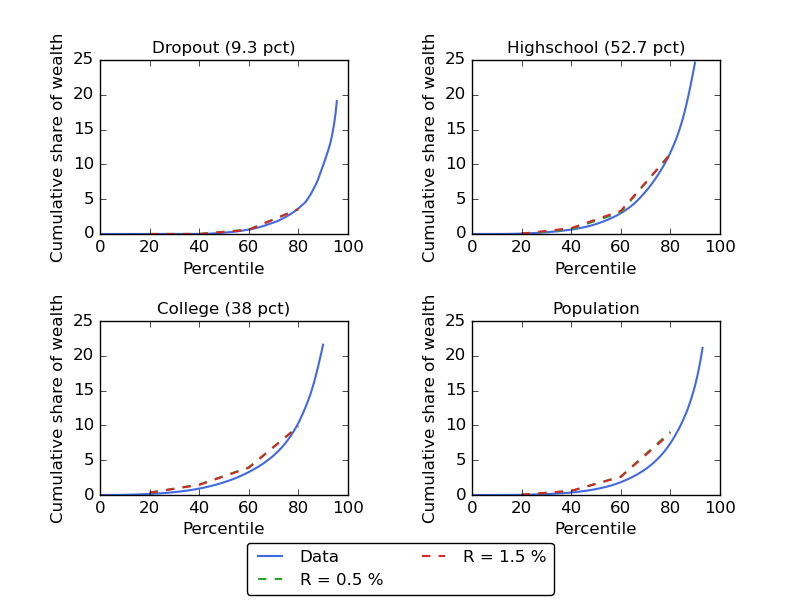
\includegraphics[width=.9\textwidth]{\econtexRoot/Figures/LorenzPoints_robustness_R}
%    \caption{Distributions of liquid wealth within each educational group and for the whole population from the 2004 Survey of Consumer Finance and from the estimated model for different values of the interest rate, $R$.}
%    \notinsubfile{\label{fig:LorenzPtsrobustnessR}}
%  \end{center}
%\end{figure}
%
%
%
%\FloatBarrier

\hypertarget{Model_without_splurge}{}\par\section{Results in a model without the splurge}
\notinsubfile{\label{app:Model_without_splurge}}

In this appendix, we consider the implications for our results of removing splurge consumption from the model.
First, we discuss that model's ability to match the empirical targets that we used to estimate the splurge in section~\ref{sec:splurge}.
Second, we repeat the estimation of discount factor distributions in the US model in section~\ref{sec:estimBetas}, and discuss the implications for both targeted and untargeted moments.
Finally, we use the reestimated model to asses the relevance of the splurge for the effectiveness of the three policies.


\subsection{Matching the IMPCs without the splurge}
%{Estimating discount factor distributions in the absence of the splurge}

For the purpose of evaluating the results in the model without the splurge we do not require the reestimation of our Norwegian model, as the purpose of the latter is the estimation of the splurge.
Nevertheless, we test how well the model can match the dynamics of spending after a temporary income shock as reported by \citet{fagereng_mpc_2021} when the splurge is zero.
Figure~\ref{fig:splurge0_Norwayestimation} illustrates the fit without the splurge and compares it to our baseline estimation.


\begin{figure}[htb]
	\centering
	\begin{subfigure}[b]{.48\linewidth}
		\centering
		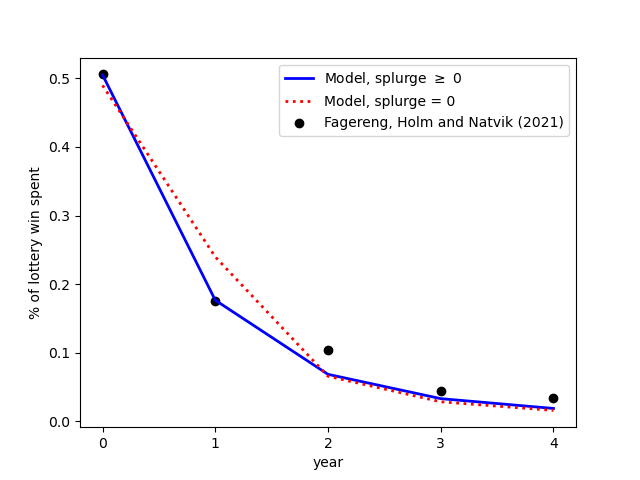
\includegraphics[width=\linewidth]{\econtexRoot/Code/HA-Models/Target_AggMPCX_LiquWealth/Figures/AggMPC_LotteryWin_comparison_splurge0}
		\caption{Share of lottery win spent}
		\notinsubfile{\label{fig:aggmpclotterywin}}
	\end{subfigure}
	\begin{subfigure}[b]{.48\linewidth}
		\centering
		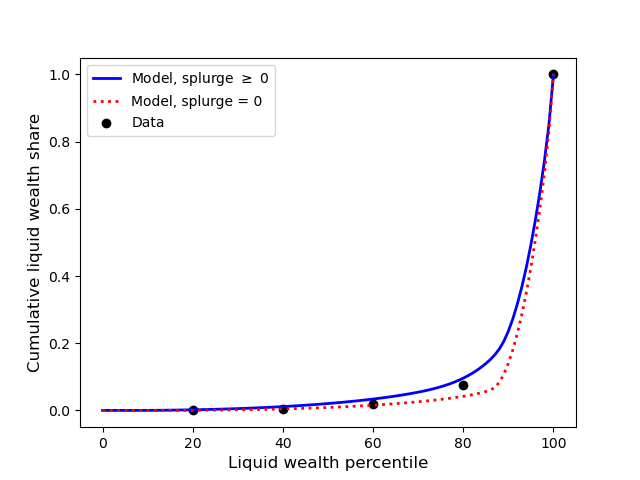
\includegraphics[width=\linewidth]{\econtexRoot/Code/HA-Models/Target_AggMPCX_LiquWealth/Figures/LiquWealth_Distribution_comparison_splurge0}
		\caption{Distribution of liquid wealth}
		\notinsubfile{\label{fig:liquwealthdistribution}}
	\end{subfigure}%
	\caption{Targets and model moments from the estimation}
	\notinsubfile{\label{fig:splurge0_Norwayestimation}}
	\parbox{16cm}{\small \vspace{.15cm} \textbf{Note}: Panel (a) shows the fit of the model to the dynamic consumption response estimated in \citet{fagereng_mpc_2021}; see their figure~A5.
Panel (b) shows the fit of the model to the distribution of liquid wealth (see Section~\ref{sec:SCFdata} for the definition) from the 2004 SCF.\normalsize}
\end{figure}

While the splurge helps in matching the empirical evidence on the IMPC, the model without the splurge also performs relatively well.
This is because the model without the splurge is able to generate a high initial marginal propensity to consume through a wider distribution of discount factors ($\beta = 0.921$ and $\nabla=0.116$) relative to the model with a splurge ($\beta = 0.968$ and $\nabla=0.0578$).
This ensures that sufficiently many agents are at the borrowing constraint and thus sensitive to transitory income shocks.

However, the model is not quite able to match the difference in spending between the initial year of the lottery win and the year after.
The model without the splurge exhibits a higher spending propensity in the year after the shock occurs as borrowing-constrained agents spend the additional income quicker.
The model without the splurge also provides a worse fit of the distribution of liquid wealth.
Relative to the baseline model, and to the data, the model without a splurge generates a more unequal wealth distribution.


The reason for these two effects, becomes apparent when considering the cross-sectional implications of the models with and without the splurge across different wealth quartiles.
While the model with the splurge can account for the empirically-observed initial MPCs among the wealthiest, the model without the splurge exhibits much lower MPCs among that group, see Table~\ref{tab:Comparison_Splurge_Table}.
The wealthiest group will thus be very patient and have low MPCs, which can explain why the wealth distribution becomes more unequal and doesn\t quite fit the targeted distribution in the data in the version of the model without the splurge.


Overall, the model fit with the data deteriorates roughly by a factor of two measured by the Euclidean norm of the targeting error.\footnote{Specifically, the Euclidean norm of the targeting error increases from 0.04 to 0.08 for the time-profile of the marginal propensity to consume when the splurge is removed, from 0.16 to 0.29 for the marginal propensity to consume across wealth quartiles and from 0.027 to 0.032 for the Lorentz curve.} 

\begin{table}[t]
	\center
	\begin{tabular}{@{}lcccccc@{}} 
\toprule 
                  & \multicolumn{5}{c}{MPC} &   \\   
                  &  1st WQ  & 2nd WQ  & 3rd WQ & 4th WQ  & Agg  &  K/Y  \\  \midrule 
Splurge $\geq$ 0 &0.27 & 0.48 & 0.60 & 0.66 & 0.50 & 6.58 \\ 
Splurge = 0 &0.13 & 0.51 & 0.62 & 0.68 & 0.49 & 6.59 \\ 
Data &0.39 & 0.39 & 0.55 & 0.66 & 0.51 & 6.60 \\ 
\end{tabular}  

	\caption{Marginal propensities to consume across wealth quartiles and the total population as well as the wealth to income ratio, in the model with and without the splurge and according to the data}
	\notinsubfile{\label{tab:Comparison_Splurge_Table}}
\end{table}

\subsection{Estimating discount factor distributions without the splurge}

Figure~\ref{fig:LorenzPtsSplZero} shows that the model without splurge consumption can also match the wealth distributions in the three education groups very well.
We therefore turn to the implications of this version of the model for the untargeted moments discussed in section~\ref{sec:nonTargetedMoments}.


\begin{figure}[th]
	\begin{center}
		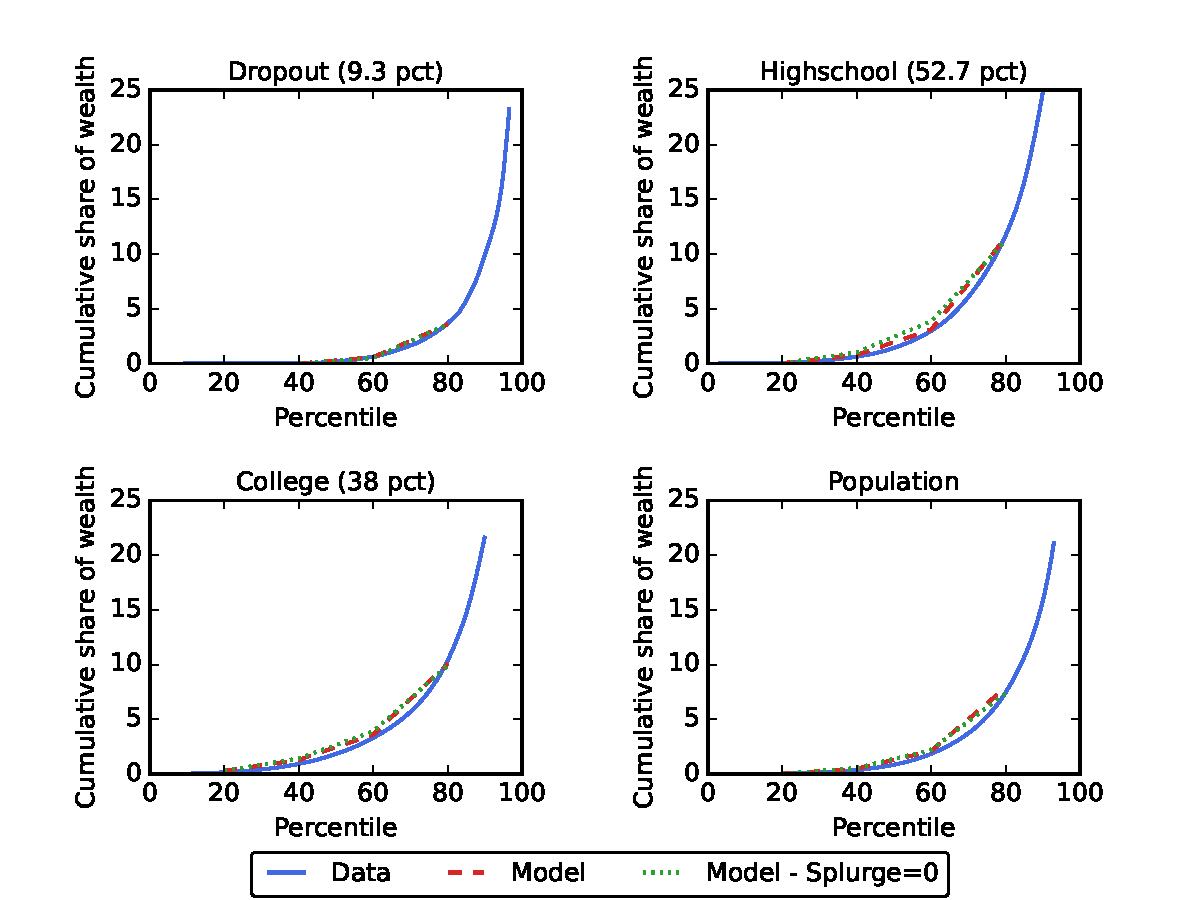
\includegraphics[width=.9\textwidth]{\econtexRoot/Figures/LorenzPoints_CRRA_2.0_R_1.01_wSplZero.pdf}
		\caption{Distributions of liquid wealth within each educational group and for the whole population from the 2004 Survey of Consumer Finances and from the estimated model withiout splurge consumption}
		\notinsubfile{\label{fig:LorenzPtsSplZero}}
	\end{center}
\end{figure}

The main difference between the models with and without splurge consumption is that without splurge consumption the MPCs drop for each education group and wealth quartile.
The difference is largest for the College group and for the highest wealth quartile (obviously with substantial overlap between these two groups).
This is shown in the two panels in Table~\ref{tab:nonTargetedMoments_wSplZero}.
The rest of the table shows that the distribution of wealth is not substantially different in the model estimated without splurge consumption.


\begin{table}[th]
	\begin{center}
		\begin{tabular}{l}
			\begin{tabular}{lcccc}
				\multicolumn{5}{l}{Panel (A) Non-targeted moments by education group} \\ \midrule
				& Dropout & Highschool & College & Population \\ \midrule
				Percent of liquid wealth (data) & 0.8 & 17.9 & 81.2 & 100 \\
				Percent of liquid wealth (model, baseline) & 1.2 & 20.1 & 78.7 & 100 \\
				Percent of liquid wealth (model, Splurge=0) & 1.6 & 18.7 & 79.7 & 100 \\
				\makecell[l]{Avg. lottery-win-year MPC \\ (model, incl. splurge)} & 0.78 & 0.63 & 0.44 & 0.54 \\ 
				\makecell[l]{Avg. lottery-win-year MPC \\ (model, splurge=0)} & 0.70 & 0.53 & 0.23 & 0.43
				\\ \bottomrule 
			\end{tabular} \\ \\ 
			
			\begin{tabular}{lcccc}
				\multicolumn{5}{l}{Panel (B) Non-targeted moments by wealth quartile} \\ \midrule
				& WQ 4 & WQ 3 & WQ 2 & WQ 1 \\ \midrule
				Percent of liquid wealth (data) & 0.14 & 1.60 & 8.51 & 89.76 \\
				Percent of liquid wealth (model, baseline) & 0.09 & 0.96 & 4.55 & 94.40 \\
				Percent of liquid wealth (model, Splurge=0) & 0.10 & 1.07 & 4.24 & 94.60 \\
				\makecell[l]{Avg. lottery-win-year MPC \\ (model, incl. splurge)} & 0.78 & 0.63 & 0.44 & 0.31 \\
				\makecell[l]{Avg. lottery-win-year MPC \\ (model, splurge=0)} & 0.69 & 0.53 & 0.36 & 0.14
				\\ \bottomrule 
			\end{tabular}
		\end{tabular}
		\caption{Implications for non-targeted moments}
		\notinsubfile{\label{tab:nonTargetedMoments_wSplZero}}
		\parbox{16cm}{\small \vspace{.15cm} \textbf{Note}: Panel (A) shows percent of liquid wealth held by each education group in the 2004 SCF and in the model.
It also shows the average MPCs after a lottery win for each education group.
The MPCs are calculated for each individual for the year of a lottery win, taking into account that the win takes place in a random quarter of the year that differs across individuals.
The MPCs are averaged across individuals within each education group.
Panel~(B) shows the same numbers for the population sorted into different quartiles of the liquid wealth distribution.\normalsize}
	\end{center}
\end{table}

%\begin{table}[th]
%	\begin{center}
%		\begin{tabular}{lccc}
%			\multicolumn{4}{l}{Model with Splurge=0} \\ \midrule
%			& Dropout & Highschool & College \\ \midrule
%			$(\beta_e, \nabla_e)$ & (0.700, 0.339) & (0.899, 0.106) & (0.978,0.019) \\
%			(Min, max) in approximation & (0.409, 0.991) & (0.809, $0.990$) & (0.962, 0.993) \\
%			\midrule 
%		\end{tabular}
%	\caption{Estimated discount factor distributions}
%		\notinsubfile{\label{tab:estimBetasSplZero}}
%		\parbox{16cm}{\small \vspace{.15cm} \textbf{Note}: Estimated parameters of the discount factor distributions for each education group in the model without splurge consumption. In parentheses are the minimum and maximum values we use in our discrete approximation to the uniform distribution of discount factors for each group. \normalsize}
%	\end{center}
%\end{table}

Finally, we again consider the  implications of our model for the dynamics of spending over time and for the dynamics of spending for households that remain unemployed long enough for unemployment benefits to expire.
Figure~\ref{fig:untargetedMoments_wSplZero} repeats Figure~\ref{fig:untargetedMoments} with results from the model without splurge consumption added.
The implication is that the model without a splurge leads to a slightly too low MPC in the year of a lottery win and a slightly higher MPC in the year after.


The drop in spending when unemployment benefits expire is virtually the same in the model without splurge consumption (17 percent versus 18 percent in the baseline).
While the consumption dynamics across the models with and without a splurge are fairly similar, the underlying drivers of the consumption drop upon expiry of unemployment benefits are different.
In the model with the splurge, the drop in income translates directly into lower consumption via the splurge itself.
In the model without the splurge it is the sharp rise in agents hitting the borrowing constraint which accounts for the consumption drop after UI benefits expire.
This is shown in the solid and dashed red lines in Figure~\ref{fig:expiryUI_wSplZero}, and is due to the wider distribution of discount factors that is needed to match the wealth distributions in the model without the splurge.
This leads to a greater number of agents being close the borrowing constraint.

\begin{figure}[thb]
	\centering
	\begin{subfigure}[b]{.48\linewidth}
		\centering
		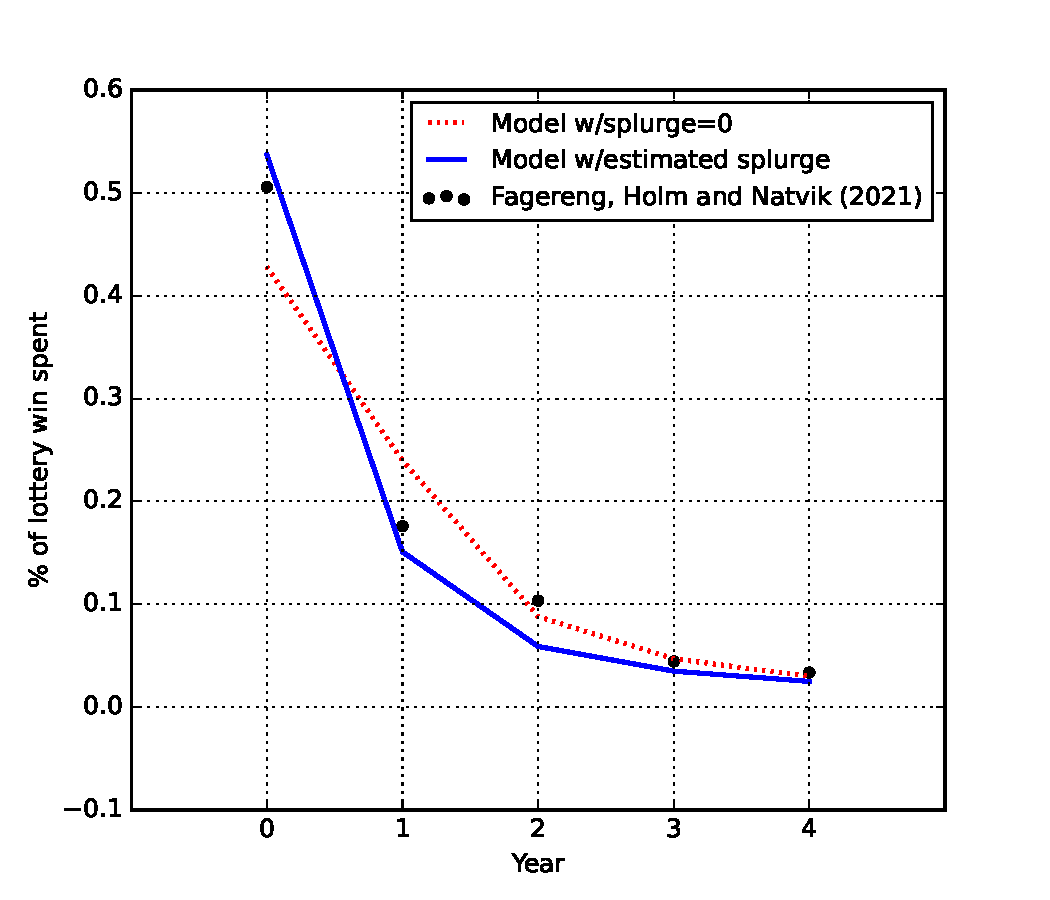
\includegraphics[width=\linewidth]{\econtexRoot/Figures/IMPCs_both}
		\caption{Share of lottery win spent}
		\notinsubfile{\label{fig:USaggmpclotterywin_wSplZero}}
	\end{subfigure}
	\begin{subfigure}[b]{.48\linewidth}
		\centering
		\includegraphics[width=\linewidth]{\econtexRoot/Code/HA-Models/FromPandemicCode/Figures/Splurge0/UIextension_CompSplurge0}
		\caption{Spending upon expiry of UI benefits}
		\notinsubfile{\label{fig:expiryUI_wSplZero}}
	\end{subfigure}%
	\caption{Untargeted moments}
	\notinsubfile{\label{fig:untargetedMoments_wSplZero}}
	\parbox{16cm}{\small \vspace{.15cm} \textbf{Note}: Panel (a) compares the dynamic consumption response in the model to the estimates in \citet{fagereng_mpc_2021}; see their Figure~A5.
Panel (b) shows the evolution of income and spending for households who remain unemployed long enough for UI benefits to expire; see Figure~2 in \citet{ganongConsumer2019}.\normalsize}
\end{figure}

%\begin{figure}[t]
%	\centering
%	\includegraphics[width=0.8\linewidth]{Code/HA-Models/FromPandemicCode/Figures/Splurge0/UIextension_CompSplurge0}
%	\caption{Consumption and income levels for agents staying unemployed for at least five quarters and the share of those agents at the borrowing limit, in the model with and without the splurge. Note: No policy nor the recession are active.}
%	\notinsubfile{\label{fig:UIextension_CompSplurge0}}
%\end{figure}


\FloatBarrier
\subsection{Multipliers in the absence of the splurge}

In this section we simulate the three fiscal policies from the main text in the estimated model without the splurge.
The shape of the impulse response functions only marginally change relative to the model with the splurge.
Hence, we focus on the quantitative changes as summarized by the cummulative multipliers in Figure \ref{fig:cumulativemultipliers_SplurgeComp}.
The figure shows the multipliers when AD effects are switched on for the model with and without the splurge.
Table \ref{tab:Multiplier_SplurgeComp} shows the 10y-horizon multiplier across the two models.

The absence of the splurge entails a calibration with a lower average MPC in the population.
Hence, the check and tax cut exhibit lower multipliers when there is no splurge.
For the UI extension we observe the opposite pattern, as the multiplier is larger in the model without the splurge.
This due to the consumption dynamics around the expiry of UI benefits described in the previous section.
In the model without the splurge more agents hit the borrowing constraint upon the expiry of benefits.
Providing those agents with an extension of UI benefits thus turns out to be slightly more powerful.


The policy ranking in terms of the multiplier shifts slighlty.
In the model with the splurge, the check policy delivers multiplier effects much more rapidly than the UI extension.
In the model without splurge consumption, the UI extension appears superior to the check, both at shorter and longer horizons.
Both models agree on the tax cut being the least effective policy.


\begin{figure}[t]
	\centering
	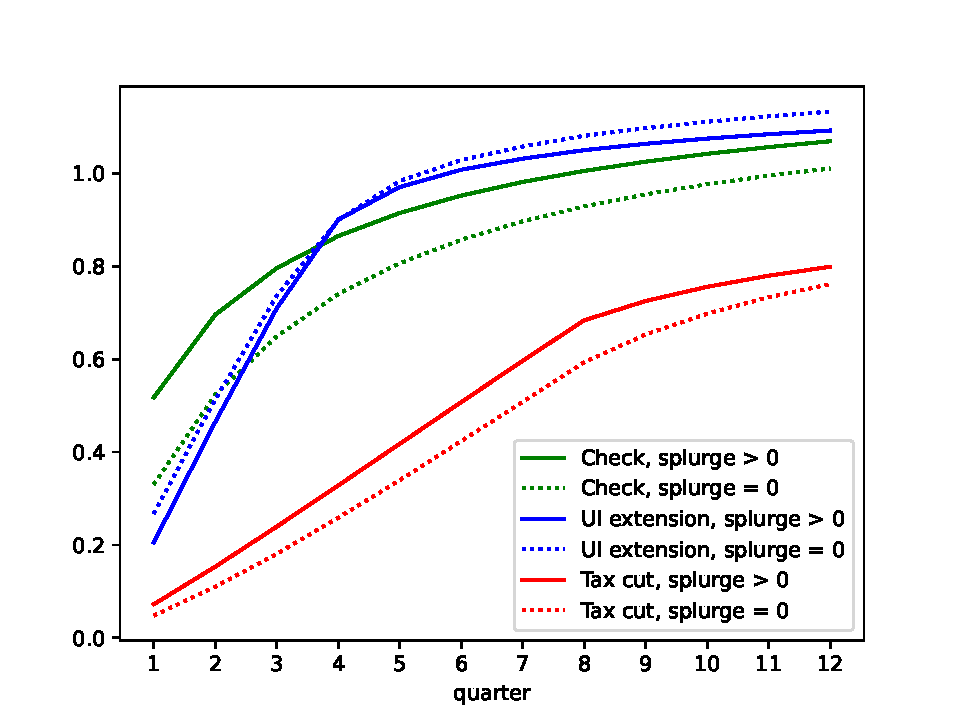
\includegraphics[width=0.8\linewidth]{Code/HA-Models/FromPandemicCode/Figures/Splurge0/Cummulative_multipliers_SplurgeComp}
	\caption{Cumulative multiplier as a function of the horizon for the three policies with and without the splurge. Note: Policies are implemented during a recession with AD effect active.}
	\notinsubfile{\label{fig:cumulativemultipliers_SplurgeComp}}
\end{figure}


\begin{table}[t]
	\center
	\begin{tabular}{@{}lccc@{}} 
\toprule 
& Stimulus check    & UI extension    & Tax cut     \\  \midrule 
10y-horizon Multiplier (no AD effect)  &0.870(0.879)  & 0.910(0.906)  & 0.839(0.847)     \\ 
10y-horizon Multiplier (AD effect) &1.143(1.234)  & 1.221(1.211)  & 0.947(0.978)     \\ 
\end{tabular}  
tabular}  

	\caption{Multipliers, calculated for policies implemented in a recession with and without aggregate demand effects. The values outside of the brackets capture the multipliers in the model without the splurge, while those inside the brackets are the corresponding mulitipliers with the splurge.}
	\notinsubfile{\label{tab:Multiplier_SplurgeComp}}
\end{table}





%\subfile{Robustness}
\subfile{Appendix-HANK}

\ifthenelse{\boolean{Web}}{}{
\end{document} \endinput
}

